\section{\ac{UML}-Verhaltesnmodelle}
\subsection{Zustandsdiagramm "Nothaltesystem"}
\begin{figure}[H]
    \centering
    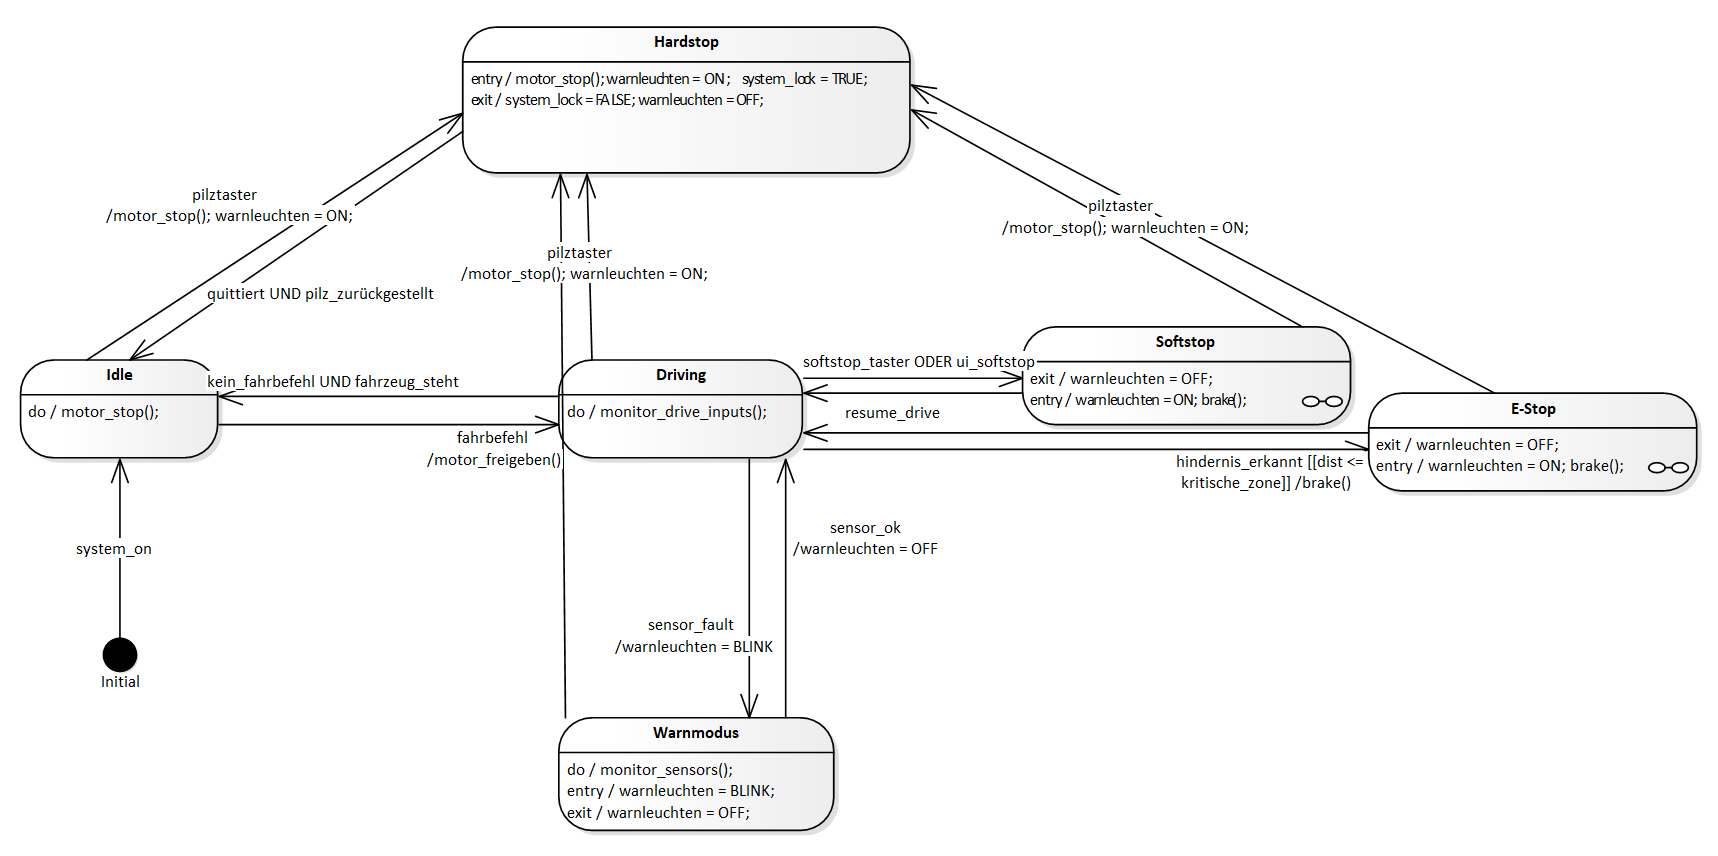
\includegraphics[width = \imglarge]{images/Nothalt_Zustandsdiagramm.png}
    \caption{Zustandsdiagramm des Nothaltesystems}
    \label{fig:zustandsdiagramm_nothalt}
\end{figure}


Das Zustandsdiagramm beschreibt das dynamische Verhalten des Nothaltesystems und
zeigt, wie es auf interne und externe Ereignisse reagiert. Im Mittelpunkt stehen
die sicherheitskritischen Zustände \ac{Hardstop}, \ac{Softstop}, \ac{E-Stop}, Idle, Driving und
Warnmodus. Jeder Zustand besitzt spezifische Entry- und Exit-Aktionen mit direkter
Auswirkung auf Motorsteuerung, Warnsignale und Systemlogik.

Ziel der Modellierung ist es, das deterministische Verhalten des Systems
transparent und prüfbar zu machen, insbesondere die Priorisierung von \ac{Hardstop}
und \ac{E-Stop} gegenüber normalen Fahrzuständen.

\paragraph{Initialer Zustand}
Nach dem Einschalten des Systems (\textit{system\_on}) wird automatisch der
Zustand \textbf{Idle} eingenommen. Dies entspricht einem sicheren Grundzustand,
in dem die Motorsteuerung deaktiviert bleibt.


% =====================================================================
\paragraph{Zustand: Idle}

\textbf{Aktionen:}
\begin{itemize}
    \item do / motor\_stop();
\end{itemize}

Der Idle-Zustand repräsentiert einen sicheren Ruhezustand. Das Fahrzeug ist nicht
freigegeben und kann keine Bewegungsbefehle ausführen.

\textbf{Übergänge:}
\begin{itemize}
    \item system\_on → Idle
    \item fahrbefehl \textbf{UND} fahrzeug\_steht → Driving
    \item pilztaster → \ac{Hardstop}
    \item sensor\_fault → Warnmodus
    \item quittiert \textbf{UND} pilz\_zurückgestellt → Idle
\end{itemize}


% =====================================================================
\paragraph{Zustand: Driving}

\textbf{Aktionen:}
\begin{itemize}
    \item do / monitor\_drive\_inputs();
\end{itemize}

Im Driving-Zustand werden Fahrzeugbewegungen erlaubt und die Fahrbefehle
kontinuierlich überwacht.

\textbf{Übergänge:}
\begin{itemize}
    \item pilztaster $\to$ \ac{Hardstop}
    \item softstop\_taster \textbf{ODER} ui\_softstop $\to$ \ac{Softstop}
    \item hinderis\_erkannt \textbf{UND} dist $\leq$ kritische\_zone $\to$ \ac{E-Stop}
    \item kein\_fahrbefehl \textbf{UND} fahrzeug\_steht $\to$ Idle
    \item sensor\_fault $\to$ Warnmodus
\end{itemize}


% =====================================================================
\paragraph{Zustand: \ac{Hardstop}}

\textbf{Entry:}
\begin{itemize}
    \item motor\_stop()
    \item warnleuchten = ON
    \item system\_lock = TRUE
\end{itemize}

\textbf{Exit:}
\begin{itemize}
    \item system\_lock = FALSE
    \item warnleuchten = OFF
\end{itemize}

Der \ac{Hardstop} ist der sicherste und restriktivste Zustand. Er kann nur manuell
ausgelöst werden und verriegelt das System, bis der Pilztaster zurückgestellt
und der Nothalt quittiert wurde.

\textbf{Übergänge:}
\begin{itemize}
    \item quittiert \textbf{UND} pilz\_zurückgestellt → Idle
    \item Von jedem Zustand erreichbar über: pilztaster
\end{itemize}


% =====================================================================
\paragraph{Zustand: Softstop}

\textbf{Entry:}
\begin{itemize}
    \item warnleuchten = ON
    \item brake()
\end{itemize}

\textbf{Exit:}
\begin{itemize}
    \item warnleuchten = OFF
\end{itemize}

Der Softstop ist ein kontrollierter Stopp ohne Systemverriegelung. Er kann über
seitlichen Taster oder UI ausgelöst werden.

\textbf{Übergang zurück:}
\begin{itemize}
    \item resume\_drive → Driving
\end{itemize}


% =====================================================================
\paragraph{Zustand: E-Stop}

\textbf{Entry:}
\begin{itemize}
    \item warnleuchten = ON
    \item brake()
\end{itemize}

\textbf{Exit:}
\begin{itemize}
    \item warnleuchten = OFF
\end{itemize}

Der \ac{E-Stop} wird automatisch ausgelöst, wenn ein Hindernis in der kritischen Zone
erkannt wird. Er stoppt das Fahrzeug unmittelbar, verriegelt das System jedoch
nicht wie ein \ac{Hardstop}.

\textbf{Übergänge:}
\begin{itemize}
    \item Nach Verlassen der Gefahr → Driving oder Idle
\end{itemize}


% =====================================================================
\paragraph{Zustand: Warnmodus}

\textbf{Aktionen:}
\begin{itemize}
    \item do / monitor\_sensors();
    \item entry / warnleuchten = BLINK;
    \item exit / warnleuchten = OFF;
\end{itemize}

Der Warnmodus wird aktiviert, wenn ein Sensorfehler auftritt. Das Fahrzeug bleibt
stehen und signalisiert eine Störung.

\textbf{Übergänge:}
\begin{itemize}
    \item sensor\_ok → Driving
    \item sensor\_ok \textbf{UND} kein\_fahrbefehl → Idle
\end{itemize}


% =====================================================================
\paragraph{Übergreifende Priorisierung}

Das Zustandsmodell definiert eine klare Priorität der sicherheitskritischen
Reaktionen:

\begin{enumerate}
    \item \ac{Hardstop} (manuell, höchste Priorität)
    \item Emergency Stop (automatisch, sicherheitskritisch)
    \item \ac{Softstop} (kontrolliert durch Operator/UI)
    \item Warnmodus (bei Sensorfehlern)
    \item Driving / Idle (Normalbetrieb)
\end{enumerate}

Diese Priorisierung stellt sicher, dass jederzeit die sicherste Reaktion ausgeführt
wird – unabhängig vom aktuellen Betriebszustand des Fahrzeugs.

\subsubsection{Interner Zustandsautomat "Softstop"}
\begin{figure}[H]
    \centering
    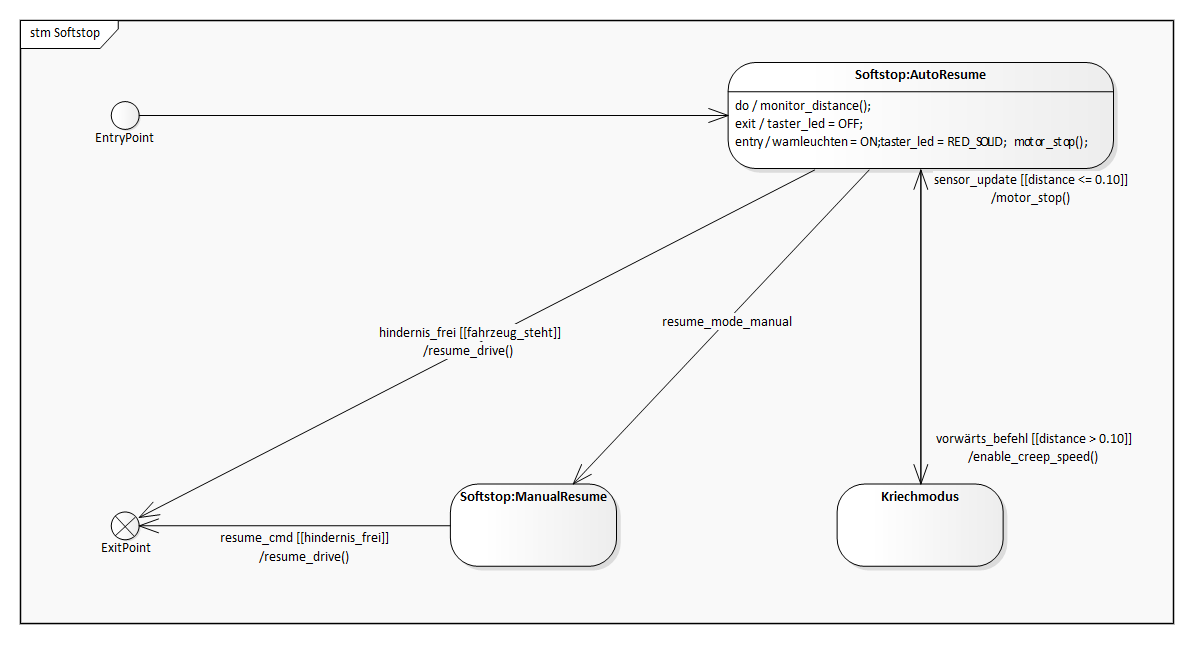
\includegraphics[width = \imglarge]{images/Softstop.png}
    \caption{Zustandsdiagramm des Softstop-Moduls}
    \label{fig:zustandsdiagramm_softstop}
\end{figure}

Der Softstop-Zustand besitzt eine eigene, hierarchische Zustandsmaschine, die den
Ablauf der Wiederaufnahme des Fahrbetriebs (AutoResume und ManualResume) sowie
den Übergang in den Kriechmodus detailliert beschreibt. Diese interne Finite
State Machine (FSM) verhindert unkontrolliertes Wiederanfahren und stellt sicher,
dass das Fahrzeug erst dann weiterfahren darf, wenn die Umgebungssituation
sicher ist.

\textbf{Startpunkt}\\
Nach Eintritt in den Softstop-Zustand beginnt die Ausführung im Zustand
\textit{Softstop::AutoResume}.

% ----------------------------------------------------------------------
\paragraph{Zustand: Softstop::AutoResume}

\textbf{Entry-Aktionen:}
\begin{itemize}
    \item warnleuchten = ON
    \item taster\_led = RED\_SOLID
    \item motor\_stop()
\end{itemize}

\textbf{Do-Aktion:}
\begin{itemize}
    \item monitor\_distance() (kontinuierliche Hindernisüberwachung)
\end{itemize}

\textbf{Exit-Aktion:}
\begin{itemize}
    \item taster\_led = OFF
\end{itemize}

Dieser Zustand versucht automatisch festzustellen, ob nach dem Softstop die
Weiterfahrt sicher möglich ist. Die automatische Wiederaufnahme wird aktiviert,
wenn keine Hindernisse mehr in unmittelbarer Nähe erkannt werden.

\textbf{Übergänge:}
\begin{enumerate}
    \item sensor\_update [distance <= 0.10] → Self-loop zu AutoResume\\
    Hindernis ist zu nah → Fahrzeug bleibt weiterhin gestoppt.

    \item hindernis\_frei \textbf{UND} fahrzeug\_steht → ExitPoint → Driving\\
    Aktion:
    \begin{itemize}
        \item resume\_drive()
    \end{itemize}

    \item resume\_mode\_manual → Softstop::ManualResume\\
    Wenn der Operator manuell übernehmen möchte (z. B. durch UI-Eingabe).

    \item vorwärts\_befehl [distance > 0.10] → Kriechmodus\\
    Der Operator fordert eine kleine Vorwärtsbewegung an → Aktivierung des Kriechmodus.
\end{enumerate}

% ----------------------------------------------------------------------
\paragraph{Zustand: Softstop::ManualResume}

Dieser Zustand erlaubt eine manuelle Wiederaufnahme durch den Operator.

\textbf{Übergänge:}
\begin{itemize}
    \item resume\_cmd [hindernis\_frei] → ExitPoint → Driving\\
    Aktion:
    \begin{itemize}
        \item resume\_drive()
    \end{itemize}
\end{itemize}

Der Operator bestätigt also aktiv, dass die Umgebung frei ist.

% ----------------------------------------------------------------------
\paragraph{Zustand: Kriechmodus}

Dieser Zustand ermöglicht eine kontrollierte, stark reduzierte Bewegung des
Fahrzeugs, z. B. wenn der Operator millimetergenau an ein Objekt heranfahren
möchte.

\textbf{Eintrittsaktion:}
\begin{itemize}
    \item enable\_creep\_speed()
\end{itemize}

Der Kriechmodus endet mit einem Fahrbefehl oder dem Verlassen des
Softstop-Hauptzustandes.

\subsubsection{Interner Zustandsautomat "E-Stop"}
\begin{figure}[H]
    \centering
    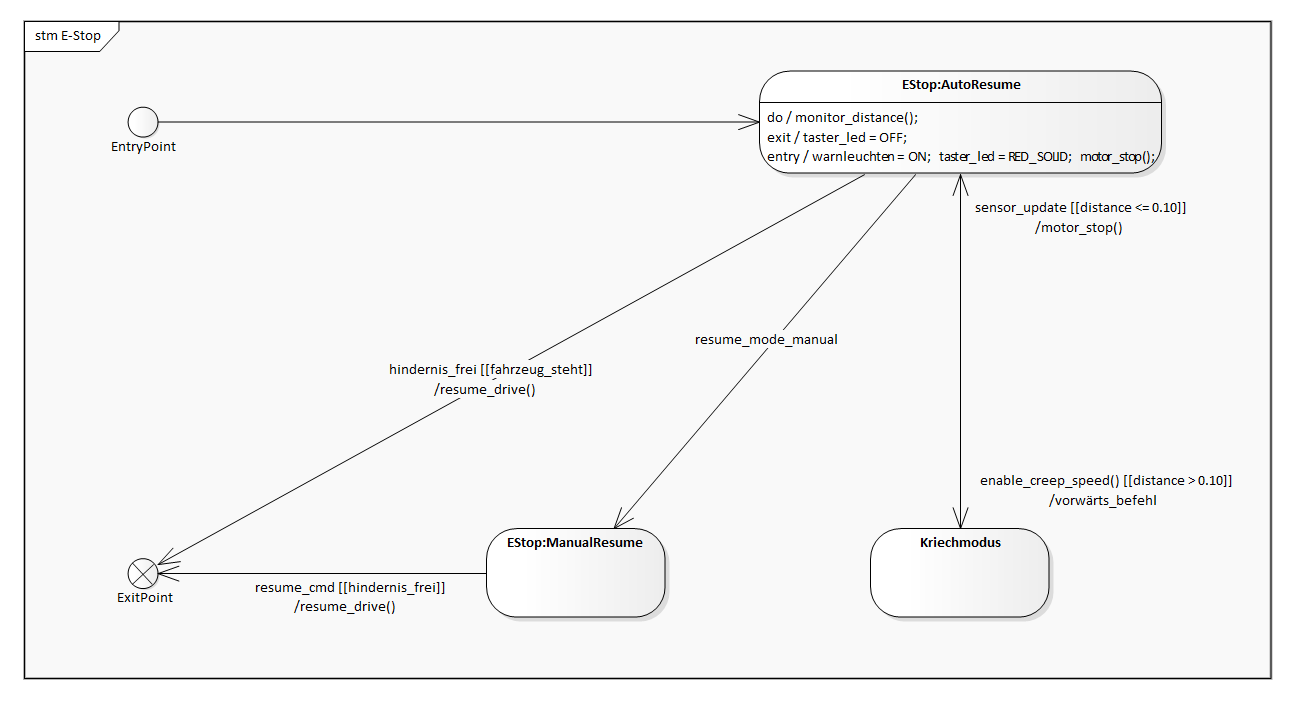
\includegraphics[width = \imglarge]{images/E-Stop.png}
    \caption{Zustandsdiagramm des E-Stop-Moduls}
    \label{fig:zustandsdiagramm_estop}
\end{figure}

Das interne Verhalten des E-Stop-Zustands entspricht strukturell dem
Softstop-Automaten, ist jedoch sicherheitskritischer. Insbesondere ist der
automatische Wiederanlauf restriktiver. Das Modell zeigt, wie das System
zwischen automatischer Wiederaufnahme, manueller Wiederaufnahme und
Kriechmodus unterscheidet.

\textbf{Startpunkt}\\
Nach Eintritt in den E-Stop-Zustand beginnt die interne FSM im Zustand
\textit{EStop::AutoResume}.

% ----------------------------------------------------------------------
\paragraph{Zustand: EStop::AutoResume}

\textbf{Entry-Aktionen:}
\begin{itemize}
    \item warnleuchten = ON
    \item taster\_led = RED\_SOLID
    \item motor\_stop()
\end{itemize}

\textbf{Do-Aktion:}
\begin{itemize}
    \item monitor\_distance()
\end{itemize}

\textbf{Exit-Aktion:}
\begin{itemize}
    \item taster\_led = OFF
\end{itemize}

Dieser Zustand überwacht kontinuierlich die Entfernung zum Hindernis. Im
E-Stop hat Sicherheit absolute Priorität: automatische Wiederaufnahme ist nur
unter klar definierten Bedingungen zulässig.

\textbf{Übergänge:}
\begin{enumerate}
    \item sensor\_update [distance <= 0.10] → Self-loop zu AutoResume\\
    Hindernis weiterhin in kritischer Nähe → Fahrzeug bleibt gestoppt.

    \item hindernis\_frei \textbf{UND} fahrzeug\_steht → ExitPoint → Driving\\
    Aktion:
    \begin{itemize}
        \item resume\_drive()
    \end{itemize}

    \item resume\_mode\_manual → EStop::ManualResume

    \item enable\_creep\_speed [distance > 0.10] → Kriechmodus\\
    Der Operator fordert Bewegung mit reduzierter Geschwindigkeit an.
\end{enumerate}

% ----------------------------------------------------------------------
\paragraph{Zustand: EStop::ManualResume}

Ähnlich wie beim Softstop kann der Operator aktiv entscheiden, die Fahrt wieder
aufzunehmen.

\textbf{Übergang:}
\begin{itemize}
    \item resume\_cmd [hindernis\_frei] → ExitPoint → Driving\\
    Aktion:
    \begin{itemize}
        \item resume\_drive()
    \end{itemize}
\end{itemize}

Manuelle Bestätigung ist erforderlich
